% Generated by code/scripts/report_figures.py at 2026-11-16T12:31:35Z; do not edit.
% Inputs: artifacts/cluster/runs/bench4-20261110T103706Z-1535991
\begin{figure}[t]
\centering
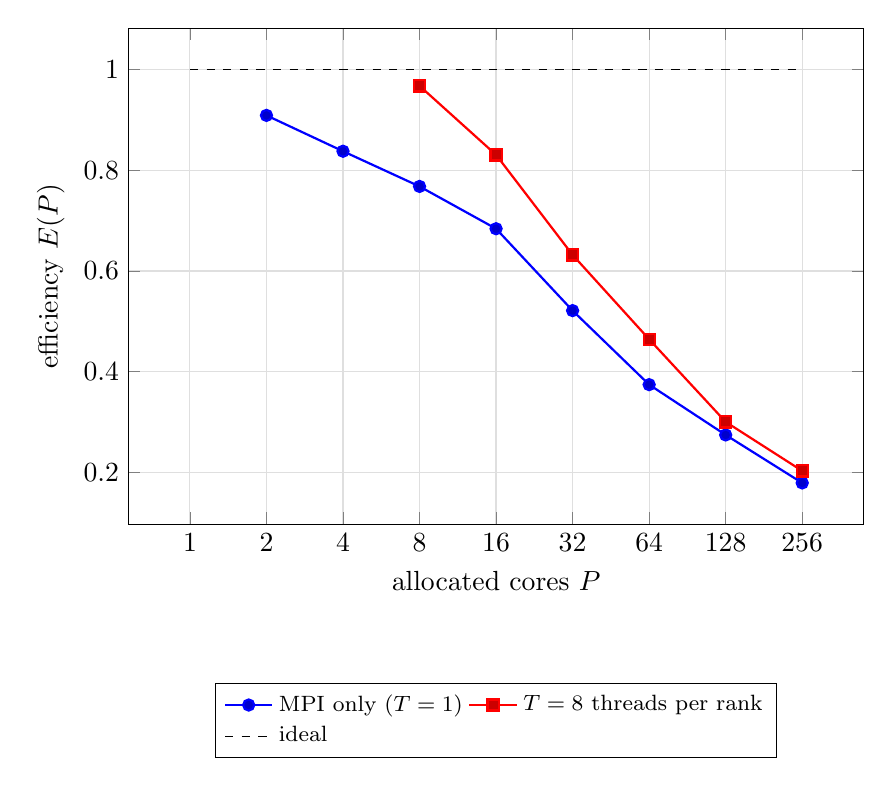
\begin{tikzpicture}
\begin{axis}[width=0.9\columnwidth, height=0.65\columnwidth, xlabel={allocated cores $P$}, ylabel={efficiency $E(P)$}, xmode=log, log basis x=2, log ticks with fixed point, legend style={at={(0.5,-0.32)}, anchor=north, legend columns=2, font=\footnotesize}, legend cell align=left, grid=major, grid style={gray!25}]
\addplot+[mark=*, thick] coordinates {(2,0.909) (4,0.8378) (8,0.7679) (16,0.6839) (32,0.5213) (64,0.3743) (128,0.2744) (256,0.1791)};
\addlegendentry{MPI only ($T=1$)}
\addplot+[mark=square*, thick] coordinates {(8,0.9676) (16,0.8306) (32,0.6319) (64,0.4644) (128,0.3003) (256,0.203)};
\addlegendentry{$T=8$ threads per rank}
\addplot[black, dashed] coordinates {(1,1) (256,1)};
\addlegendentry{ideal}
\end{axis}
\end{tikzpicture}
\caption{Strong-scaling efficiency. $N=10^{6}$, median of repetitions; serial Barnes--Hut baseline on the same CPU model and build. Vanda job 1535991: 64 of 72 cores on each of four Platinum 8452Y nodes (CN-047, CN-061, CN-064, CN-065), 3 interleaved repetitions.}
\label{fig:b4-strong-efficiency}
\end{figure}
